\chapter* {Búsqueda lineal}
\addcontentsline{toc}{chapter}{Búsqueda lineal}
\markboth{Búsqueda lineal}{Búsqueda lineal}
La búsqueda lineal es la más sencilla de las búsquedas que hay. ¿Qué es lo que harías si te pido que de una pila de exámenes encuentres el tuyo? Lo que probablemente hagas es una revisar uno por uno, checar de arriba hacia abajo hasta que encuentres el examen con tu nombre en él.

Básicamente, esta idea es la búsqueda lineal, ir revisando de uno por uno toda una lista de candidatos hasta encontrar al que estas buscando o hasta que hayas revisado todos los candidatos.

Entonces, los códigos de búsqueda lineal casi siempre tendrán la siguiente estructura:

\begin{lstlisting}
Itera por cada candidato {
	Si el candidato es lo que buscamos {
		Respuesta = candidato;
		Detener ciclo /* esto es opcional, depende si hay varios valores que queramos encontrar. */
	}
}	
\end{lstlisting}

Veamos cómo usar esta técnica para resolver un problema.

\section*{Ejemplo 1.1}
\addcontentsline{toc}{section}{Ejemplo 1.1}

\subsection*{Descripción}
Supongamos que queremos tenemos un arreglo \(A\) de enteros distintos y este tiene \(N\) elementos en él. Nosotros querremos hacer un código que imprima la posición del arreglo que valga \(K\). O si este valor no existe, que imprima \(-1\).

\subsection*{Límites}
\begin{plimits}
	\item \(1\leq N \leq 10^5\)
	\item \(1\leq K,A[i] \leq 10^9\)
\end{plimits}
\subsection*{Solución}

(Recuerda intentar el problema antes de leer la solución)

Lo que este problema nos pide en realidad es buscar dentro del arreglo por el índice del elemento \(K\).

Lo que haremos es revisar todas las posiciones del arreglo hasta encontrar aquella que valga \(K\), si no la encontramos imprimimos \(-1\).


\subsection*{Código}
\begin{lstlisting}
int A[100050];
int N, K;
int main () {	
	ios_base::sync_with_stdio(0); cin.tie(0);
	cin >> N;
	for (int  i=0; i <N; i++){ 
		cin >> A[i];
	}
	cin >> K;
	int respuesta = -1;
	for (int i =0; i < N; i++) {
		if (A[i]==K) {
			respuesta = i;
			break;
		}
	}
	cout << respuesta;
}
\end{lstlisting}


\subsection*{Complejidad}

Una pregunta que te has de hacer es: ¿cuál es la complejidad de esta técnica? Y la respuesta es sencilla, en el peor de los casos tenemos que revisar a todos los candidatos, digamos que la cantidad de ellos es iguala a \(N\), entonces la complejidad es \(O(N)\).

\section*{Ejemplo 1.2}
\addcontentsline{toc}{section}{Ejemplo 1.2}
Veamos otro problema de búsqueda lineal. 

\subsection*{Descripción}

Carlos quiere armar una fiesta, y como le gusta ser un buen anfitrión compro \(N\) regalos para sus invitados.
Ahora, Carlos quiere darle la misma cantidad de regalos a cada uno de sus invitados sin que sobre ningún regalo no repartido. Como Carlos le gusta contar, ahora se pregunta: ¿Cuántas cantidades diferentes de invitados puede tener?
\subsection*{Entrada}
Un entero \(N\), indicando cuantos regalos compró Carlos.
\subsection*{Salida}
La cantidad de posibles números de invitados para la fiesta.
\subsection*{Casos ejemplo}
\begin{casebox2}
	\scase{12}{6}
	\scase{7}{1}
	\scase{4}{3}
\end{casebox2}
\subsection*{Límites}
\begin{plimits}
	\item \(1\leq N \leq 10^5\)
\end{plimits}

\subsection*{Solución}
Es fácil ver que el problema en realidad pregunta: ¿Cuántos divisores positivos tiene \(N\)?

(Nota: un divisor de \(N\) es un número que divide a \(N\) sin decimales).

Encontremos todos los divisores de \(N\). Estos se encontrarán entre \(1\) y \(N\), por lo que podemos iterar i por todo este rango revisando si \(i\) es divisor de \(N\).
\subsection*{Código}
\begin{lstlisting}
respuesta = 0;
for (int i =1; i <= N; i++) {
	if (N%i==0) {
		respuesta++;
	}
}
cout << respuesta;
\end{lstlisting}
\newpage
\practiceproblemsection{1}

\problemtitle Dado una lista de \(N\) enteros, cuenta cuantas veces aparece el valor \(K\). 

\begin{plimits}
	\item \( 1\leq N\leq 10^5 \)
\end{plimits}

Enlace: TODO

\problembreak

\problemtitle Dado una lista de \(N\) enteros, imprime todos los múltiplos de \(5\) que estén en la lista y en el mismo orden que aparecen en la lista. 

\begin{plimits}
	\item \(1\leq N \leq 10^5\)
\end{plimits}

Enlace: [TODO]

\problembreak

\problemtitle Cuenta cuantos enteros positivos dividen a \(K\) exactamente. Similar al ejemplo, pero los límites son más grandes.
\begin{plimits}	
\item \(1\leq K \leq 10^9\)
\end{plimits}

Enlace: 3 [TODO]

\problembreak

\problemtitle Encuentra el entero más grande que sea menor o igual a R y que la suma de sus dígitos sea menor o igual que S. Se garantiza que siempre existe este entero.
\begin{plimits}
\item \(1\leq S\leq 50\)
\item \(1\leq R\leq10^5\)
\end{plimits}

Enlace: omegaup.com/arena/problem/bl-1-4 [TODO]

\problembreak

\problemtitle Fernando construye escaleras de ladrillos de la siguiente forma:
\begin{center}
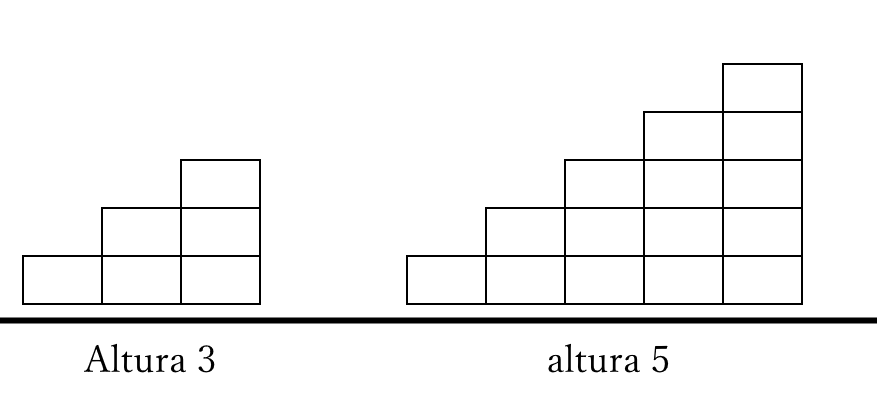
\includegraphics[scale=0.25]{escaleras}
\end{center}

El otro día, Fernando obtuvo \(K\) ladrillos, ahora se pregunta ¿Qué tan alto que puede construir una escalera? Dado \(K\), responde su pregunta.

\begin{plimits}
	\item \(1\leq K \leq 10^9\)
\end{plimits}

\subsubsection{Casos ejemplo}
\begin{casebox2}
	\scase{12}{4}
	\scase{8}{3}
	\scase{20}{5}
\end{casebox2}

Enlace: [TODO]
